\documentclass{article}


\usepackage[margin=1in]{geometry}
\usepackage{amsmath}
\usepackage{graphicx}
\usepackage{tabu}
\usepackage{float}
\usepackage{listings}
\usepackage{color}
\usepackage{caption}

\author{Zachary Vogel\quad James Pentz}
\title{Embedded Software Essentials Project 1\\ ECEN 5013}
\date{\today}

\begin{document}
\begin{titlepage}
    \centering
    \vspace*{2cm}
    {\scshape\Huge Embedded Software Essentials \par}
    \vspace{2cm}
    {\scshape\Large Project 1: Build System and Software Design \par}
    \vspace{2.5cm}
    {\Large \scshape Zachary Vogel \& James Pentz\par}
    \vspace{1cm}
    {\large \itshape Professor: Alexander Fosdick}
    \vfill
    {\large \today\par}
\end{titlepage}

\section*{Introduction}
The goal of this project is to build a BeagleBone Black Build System and then write some code to test this implementation. The goal of the makefile is to be able to use the same make to build code for the beaglebone or for a regular computer. This allows us to quickly test code on a laptop, and also quickly upload it to the board. The coding problems are just for practice and something to test.


\section*{Project Procedure Results}
To show that we had the output of various builds, we took some screenshots. These are shown below with appropriate captions.
\begin{figure}[H]
    \centering
    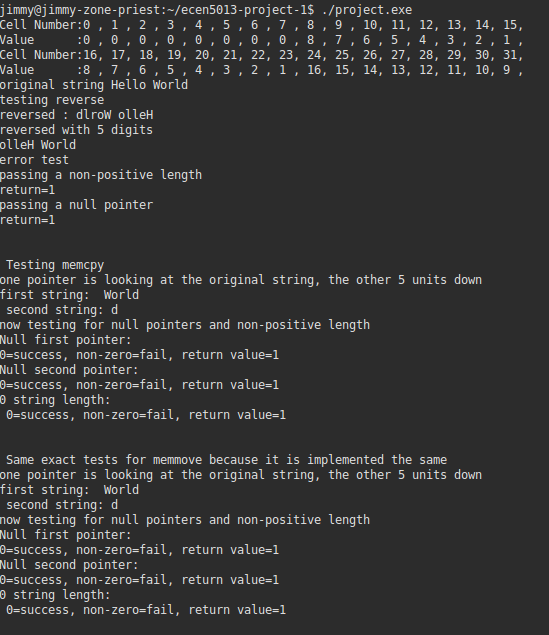
\includegraphics[width=0.8\textwidth]{x86_exe_pic1.png}
    \caption{First a photo of the output of our code on the x86 architecture. Note that this includes the running of our test function, which is everything you see after the 4th line.}
\end{figure}

\begin{figure}[H]
    \centering
    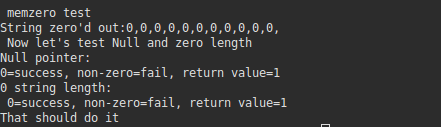
\includegraphics[width=0.8\textwidth]{x86_exe_pic2.png}
    \caption{This is the rest of the output from the previous image}
\end{figure}

\begin{figure}[H]
    \centering
    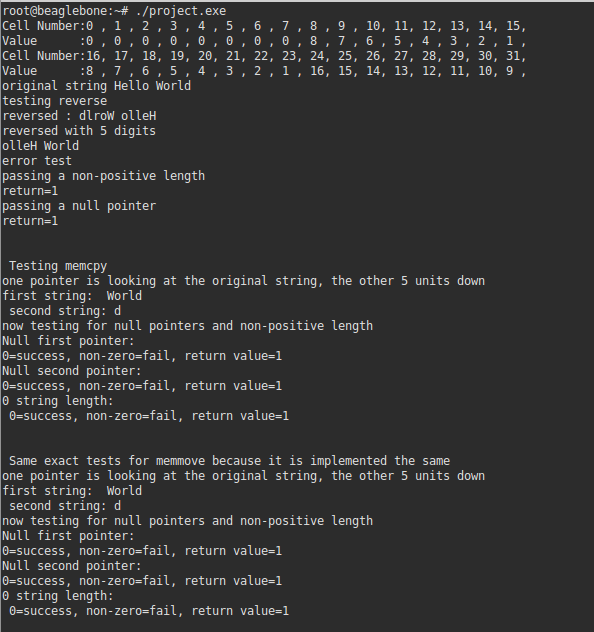
\includegraphics[width=0.8\textwidth]{beaglebone_exe_pic1.png}
    \caption{Now we see the exact same thing, but run on the beaglebone}
\end{figure}

\begin{figure}[H]
    \centering
    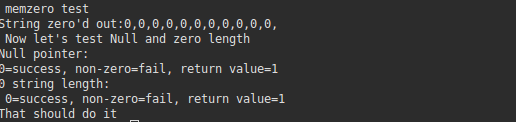
\includegraphics[width=0.9\textwidth]{beaglebone_exe_pic2.png}
    \caption{Second part of figure 3}
\end{figure}

\begin{figure}[H]
    \centering
    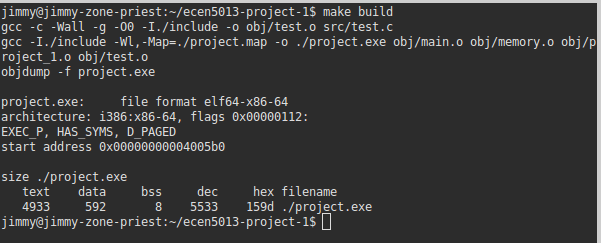
\includegraphics[width=0.9\textwidth]{make_build_all.png}
    \caption{The output of the make build command}
\end{figure}

\begin{figure}[H]
    \centering
    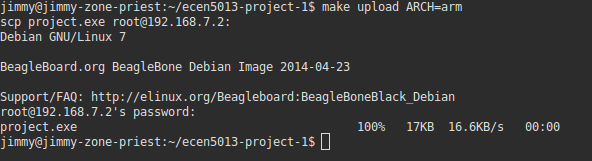
\includegraphics[width=0.9\textwidth]{scp_pic.png}
    \caption{The output of the make upload ARCH=arm command}
\end{figure}

\begin{figure}[H]
    \centering
    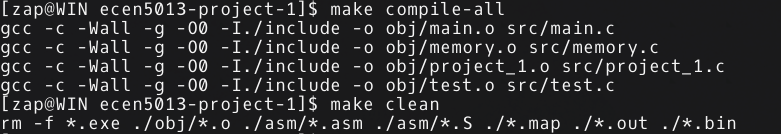
\includegraphics[width=0.9\textwidth]{other_make.png}
    \caption{The output of the make compile-all and make clean commands}
\end{figure}

As you can see requirements 1, 2, and 4-6 are completed. The testing was largely calls to make sure the functions worked, as well as testing for bad input. The main file calls two functions, project\_1 and the testing function for the memory functions memtest. We could have compiled them into seperate binaries, but decided not to. This is because it isn't a ton of output and we figured it would be better to print it all at once.

The final thing is to explain what we did for memmove and memcopy. Since the implementation details weren't that specific, our memmove is actually just a call to memcopy. memcopy itself is relatively simple, it checks for bad input and returns if it fails. Otherwise it copies everything from the first pointer into a temporary array and then copies it into the second pointer. This addresses any issues that might happen with
overlapping. Another implementation would be to check for overlap first, fail if you are doing memcopy, and then copy only the overlapping region into an array. Then, move the non-overlapping part, and finally the overlapping part. This would be more efficient in terms of memory, but is slightly more intensive in terms of coding. 

\section*{Conclusion}
We have completed everything required of us for this assignment. This included making a very generic makefile, which is generic in the sense it works on a variety of systems. We also built the functions required for this assignment properly and tested them using the memtest function call in main.c. All components of this lab can be found on James Pentz's github at jgpentz/ecen5013-project-1. It has been a decent experience, we both gained quite a bit of knowledge on makefiles. We
also gained more experience using git with 2 developers so that is nice. We were wondering if we will learn more about making makefiles that might pull code from multiple languages.

%\captionsetup{labelformat=empty}
\end{document}
